\chapter{Обзор предметной области}\label{ch:ch1}

\section{Антагонистические игры и случайные блуждания}\label{sec:ch1/sec1}

Теория игр тесно переплетается с проблемами случайных блужданий в широком спектре областей прикладных и фундаментальных исследований 
от хемотаксиса бактерий и рыночных взаимодействий до блужданий роя автономных роботов и компьютерных игр \cite{}. 
Игры, в которых возникают случай влияет на развитие игровой ситуации, могут быть рассмотрены как случайное блуждание
на некотором графе всех возможных конфигураций предметов игры или в некотором непрерывном пространстве всех возможных состояний.
В общем случае окончание таких игр определяется при возникновении некоторой предопределенной выигрышной траектории.
Одной из таких возможных ситуаций является поглощение траектории в некотором состоянии при случайном блуждании в пространстве конфигураций.
В зависимости от типа игры игрокам может требоваться оптимизировать длительность случайного блуждания или расставить поглощающие состояния 
так, чтобы раньше другого игрока поймать траекторию \cite{}. Одной из самых простых игр такого типа является задача о разорении игрока \cite{}
и различные её модификации \cite{}. Обобщение случайных блужданий игрового типа было проведено в работе И.~В.~Романовского \cite{romanovskiy_1961}.
Рассматриваемые теорией игр процессы обусловлены взаимодействием одного игрока с некоторой системой, двух игроков или множества игроков.
В последующих разделах проведен анализ первых двух случаев, соответствующих антагонистическим играм между двумя игроками с противоположными интересами.

\subsection{Задача о разорении игрока}\label{subsec:ch1/sec1/sub1}

Впервые упоминание о задаче разорения игрока появилось в переписке Блеза Паскаля и Пьера Ферма в 1656 году при рассмотрении игры тремя костями между двумя игроками.
Первый игрок получал очки при выпадении суммы на игральных костях равной $11$, а второй игрок при выпадении суммы равной $14$. Однако, способ начисления очков 
был модифицирован: очко добавляется к счету игрока только в том случае, если счет его противника равен нулю, а в противном случае очко будет вычтено из счета его противника.
В этом случае счет отстающего игрока всегда остается равным нулю. Первый из игроков набравший $12$ очков объявлялся победителем. В переформулированной версии
письма Пьером де Каркави, направленной Христиану Гюйгенсу в 1656 году, вопрос к задаче состоял в нахождении вероятности победы первого и второго игрока. 

В своей работе De ratiociniis in ludo aleae Христиан Гюйгенс получил более приближенную формулировку к классической: игроки начинают с $12$ очков, успешный бросок 
трех костей ($11$ для первого и $14$ для второго) добавляет этому игроку одно очко и вычитает у второго, при этом первый достигший нуля очков проигрывает.
Вопрос как и ранее состоял в нахождении вероятности победы игроков. 

Классическая формулировка обобщает для одномерного случая задачу о разорении игрока для случая произвольных начальных условий и произвольных вероятностей перехода. 
Пусть у первого игрока есть $-A$ монет ($A < 0, -A > 0$), у второго игрока - $B$ монет. На каждом ходу подбрасывается ассиметричная монета, имеющая вероятность выпадения 
аверса $p$ и реверса $1-p$. При выпадении аверса одна монета переходит от второго игрока к первому, при выпадении реверса - наоборот. Требуется найти вероятность проигрыша 
за $n$ шагов, а также общую вероятность проигрыша каждого из игроков. В дополнение к формулировке Христиана Гюйгенса ставится вопрос о среднем времени игры, 
где время игры характеризует количество ходов до проигрыша одного из игроков.

Тесная связь со случайными блужданиями позволяет сформулировать данный процесс в виде дискретного блуждания частицы по целочисленному отрезку $[A; B]$, 
при этом выход на границу отрезка характеризует проигрыш одного из игроков. 

Решение задачи состоит в рассмотрении схемы Бернулли с последовательностью Бернуллиевских случайных величин $\xi_i$ с вероятностью $p$ дающих $+1$ и 
с вероятностью $q=1-p$ значение $-1$.
Тогда сумма таких величин $S_k=\sum_{i=1}^{k} \xi_i$ равна случайной величине, соответствующей положению частицы в случайном блуждании на отрезке $[A; B]$.
Вводя обозначения для вероятностей завершить игру в точках $A$ и $B$ за время $[0; k]$ при старте в позиции $x$ соответственно $\alpha_k(x), \beta_k(x)$ 
запишем рекуррентные соотношения:

\begin{equation}
    \label{eq:eq1}
    \begin{alignedat}{2}
        \alpha_k(x) = p\alpha_{k-1}(x+1)+q\alpha_{k-1}(x-1),\\
        \beta_k(x) = p\beta_{k-1}(x+1)+q\beta_{k-1}(x-1).
    \end{alignedat}
\end{equation}

При достаточно больших $n$ решение рекуррентного соотношения близко к стационарной точке точечного отображения при заданных граничных условиях:
\begin{equation}
    \label{eq:eq2}
    \begin{alignedat}{2}
        \alpha(x) = p\alpha(x+1)+q\alpha(x-1), \alpha(A)=1, \alpha(B)=0,\\
        \beta(x) = p\beta(x+1)+q\beta(x-1), \beta(A)=0, \beta(B)=1.
    \end{alignedat}
\end{equation}

Поиск решения уравнения в форме $(q/p)^{x}$ дает следующий результат:
\begin{equation}
    \label{eq:eq3}
    \begin{alignedat}{2}
        \alpha(x) = ((q/p)^B-(q/p)^x)/((q/p)^B-(q/p)^A),\\
        \beta(x) = ((q/p)^x-(q/p)^A)/((q/p)^B-(q/p)^A).
    \end{alignedat}
\end{equation}

При справедливой игре $(p=q)$ выражения для определения вероятностей редуцируются до линейной формы:
\begin{equation}
    \label{eq:eq4}
    \begin{alignedat}{2}
        \alpha(x) = (B-x)/(B-A),\\
        \beta(x) = (x-A)/(B-A),
    \end{alignedat}
\end{equation}
где $x \in [A; B]$ "---- стартовое положение на отрезке.

Заключительный аспект задачи о разорении игрока состоит в исследовании среднего времени достижения финального состояния.
С точки зрения случайных блужданий процесс представляется в виде Марковской цепи с поглощающими состояниями на концах отрезка 
и промежуточными состояниями в целочисленных координатах отрезка. Рассмотрим подход к решению задачи о нахождении математического
ожидания времени окончания игры $m_k(x)$ для некоторой игры длины $k$ находящейся в состоянии $x$. Тогда рекуррентное соотношение 
для соседних состояний представляется в виде:
\begin{equation}
    \label{eq:eq5}
    m_k(x) = p m_{k-1}(x + 1) + q m_{k-1}(x - 1) + 1, x \in (A, B), k > 0,
\end{equation}

На границе в точках $A$, $B$ количество ходов для завершения игры равно нулю, то есть $m_k(A) = m_k(B) = 0$.
С учетом конечности математического ожидания пределом при $k->\infty$ будет являться решение рекуррентного соотношения 
$m(x)=p m(x+1) +q m(x - 1) + 1$. Итоговое решение для общего случая представляется в виде:

\begin{equation}
    \label{eq:eq6}
    m(x) = 1 / (p - q) (B \beta(x) + A \alpha(x) - x)
\end{equation}

При симметричной монетке формула упрощается до $m(x) = (B - x) (x - A)$, а в случае равного начального капитала $m(x) = B^2$.

Таким образом оценки позволяют найти как вероятность выигрыша каждого из игроков в зависимости от параметров игры, так и среднее время игры.

\subsection{Задача о разорении игрока с несколькими валютами}\label{subsec:ch1/sec1/sub2}

Обобщение задачи о разорении игрока на двумерный случай было рассмотрено израильскими математиками в 1994 году \cite{}. 
Для решения задачи был применен метод производящих функций и получены выражения для случая с равновероятными переходами на отрезке и на квадратной решетке.
Применяя символьные вычисления в пакете MAPLE \cite{} тем же способом было найдено решение с произвольными вероятностями перехода в 4 направлениях 
на четырех-связной решетке. 

Естественным продолжением двумерного случая является обобщение на произвольные размерности. В 2000 году Марко Петковсек и Андреем Кмет 
рассмотрели задачу о разорении игрока, в которой имеется несколько различных валют. \cite{}
Формулировка игровой механики для многомерного случая состоит в равновероятном выборе валюты и победителя на каждом ходу.
В результате хода победитель забирает одну монету выпавшей валюты у проигравшего. Игра продолжается до тех пор, пока у одного из игроков не закончатся монеты любой из валют.
В своей работе словенские математики получили среднее время игры в явной форме для случая равновероятных переходов между соседними узлами решетки
с применением дискретного преобразования Фурье и выражений для спектра симметричной тридиагональной матрицы Теплица.
Полученное выражение для среднего времени игры в зависимости от начального капитала игроков состоит из двойной суммы для двумерного случая 
и может быть вычислено за время $O(N^2)$: 
\begin{equation}
    \label{eq:eq7}
    a_{ij} = 4 / N^2 \sum_{k=1\\ k odd}^{N - 1} sin(jk\pi/N)cot(k\pi/(2N)) \\
    \sum_{l=1\\ l odd}^{N - 1} sin(il\pi/N)cot(l\pi/(2N))/(sin^2(k\pi/(2N))+sin^2(l\pi/(2N))), \\
    0 <= i, j <= N
\end{equation}
Хотя авторы не получили более быстрый алгоритм для общего случая, высказано предположение о возможности получения выражения в виде одной суммы.
Явные формулы в виде одной суммы (вычислительная сложность $O(N)$) были получены для частного случая стартовых капиталов одинакового размера являющегося степенью 2.
Также математики получили решение для многомерного случая на базе уравнения Сильвестра и тензорного спектрального разложения.

\subsection{Случайные блуждания}\label{subsec:ch1/sec1/sub3}

Первое появление термина "случайные блуждания" относится к письму Карла Пирсона в редакцию журнала Nature в 1905 году \cite{}.
Мотивированный проблемами, возникшими в биологии, он сформулировал следующую задачу:
"Человек начинает путешествие из точки $O$ и проходит $l$ ярдов по прямой линии. 
Затем он поворачивается на какой угодно угол, и проходит еще $l$ ярдов по прямой линии. 
Он повторяет этот процесс $n$ раз. Я ищу вероятность того, что после этих n прогулок он окажется 
на расстоянии между $r$ и $r+dr$ от своей начальной точки $O$."

На письмо ответил британский физик Лорд Рэлей, который ранее в своей работы 1880 года от теории звука рассмотрел
n изопериодических колебаний единичной амплитуды и фазы, распределенные случайным образом. Для достаточно больших n 
Рэлей нашёл асимптотическое решение в замкнутой форме, отражающее распределение вероятностей в задаче Карла Пирсона. 

Решение задачи для многомерного случая в евклидовом пространстве представляется существенно более сложной задачей в связи с чем в своих работах Лорд Рэлей
рассматривал модель случайного блуждания на решетке. Исследуя случайные блуждания на решетке Дьёрдь Пойа в своих работах 1919 и 1921 года \cite{} показал, что, 
в случае случайного блуждания на решетке с равновероятными переходами во всех направлениях в одномерном и двумерном случаях, 
агент возвращается в исходную точку с вероятностью $1$, а для размерностей больше двух с вероятностью $0$.

Как заметил профессор прикладной математики Невилл Темперлей, различные комбинаторные задачи, возникающие при изучении 
разнообразных физических явлений, связанных с решетками, могут быть разрешимы в терминах подсчета числа траекторий случайного блуждания с ограничениями \cite{}. 
Задачи, возникающие в различных областях таких как химия, физика, экономика, биология, сводились к анализу случайных блужданий на решетках со сложной структурой и 
особыми ограничениями \cite{, , , ...}. 

После публикации Куна в начале 20-го века все большее внимание уделялось статистике конфигураций гибких макромолекул. 
Важность исследования состояла в том, что химические свойства и биологически функции различных макромолекул напрямую 
зависят от их трехмерной пространственной конфигурации. Кун рассматривал первое приближение такой задачи 
с помощью свободно сочлененной цепи с звеньями фиксированной длины, но со случайной ориентацией, то есть задача Пирсона, но в трехмерном случае. 
Такая конструкция не учитывает тот факт, что в одной точке пространства может быть только один атом полимерной цепи. 
Упрощение задачи на случай решеток, подобно тому, как это делал Лорд Рэлей, позволяет получить решение с помощью численных методов.

Первые попытки в направлении исследования блужданий без самопересечений были сделаны В. Орром в 1946 году [61]. 
В 1924 году немецкий и американский математик Эрнст Изинг сформулировал модель ферромагнетизма на плоскости, 
для которой интересным является её соответствие случайным блужданиям без самопересечений на решетке [62]. 
В 1941 году Бартель Леендерт ван дер Варден показал, как можно свести эту задачу к подсчету числа решетчатых графов, 
состоящих из замкнутых многоугольников [63]. Знаменитое решение задачи Изинга, полученное Ларсом Онзагером, было впервые 
опубликовано 18 февраля 1942 года в дискуссионных заметках на собрании Нью-Йоркской академии наук [64]. 
Модель Изинга может быть использована для описания и других различных физических систем, таких как поглощение 
газа поверхностью или описание двухкомпонентного сплава. Эти явления описываются грубой моделью равновесия жидкости и пара на двумерной решетке.

В 1912 году Андрей Андреевич Марков разработал общую постановку задачи случайных полетов, а также предложил метод для отыскания решения [68]. 
Задача формулируется так: есть частица в трехмерном пространстве, которая совершает перемещения на каждому шаге в соответствии с некоторым распределением, 
зависящим от номера шага. Требуется найти вероятность обнаружить частицу на некотором расстоянии от позиции старта. 
Решение Маркова использует свойства преобразования Фурье.

Исследуя свойства случайных процессов в своей работе 1907 года выделил класс обладающий характеристикой независимости 
будущих состояний от прошлых состояний при определенном настоящем состоянии. В зависимости от рассматриваемой модели 
Марковские процессы могут быть обобщены на процессы с дискретным и непрерывным временем. Марковские цепи высшего порядка
в свою очередь обладают свойством зависимости перехода от последних $k$ состояний.

Анализ различных типов случайных блужданий позволил выделить множество различных объектов, на которых возможно осуществлять блуждание:
графы, числовая прямая (целые или действительные числа), векторные пространства, конечные группы, группы Ли, кривые поверхности и другие.
Случайные блуждания также различаются по типу времени: дискретное или непрерывное $(t \in [0; +\infty])$. 
Хотя в общем случае случайное блуждание не обязательно должно обладать свойством Марковости, 
по умолчанию подразумевают зависимость будущих состояний только от текущего состояния.

\subsection{Случайные блуждания игрового типа}\label{subsec:ch1/sec1/sub4}

Дальнейшие исследования игр привели к анализу многошаговых процессов, в которых игроки на каждом ходу выбирают одну из доступных стратегий \cite{}. 
Ричард Беллман в своей работе 1954 года рассматривал проблему принятия решений в многошаговых играх в условиях неопределенности \cite{} и 
привел приближенное решение задачи. Возникновение прямого конфликта позволяет использовать известные работы игр с нулевой суммой \cite{}, 
тогда как частичное противостояние требует более сложного анализа игр с ненулевой суммой \cite{}. Одной из естественно возникающих вариаций 
являются игры на выживание введенные в работах \cite{,} в 1952 году Мелвином Хауснером и Мелвином Пейсахов. В таких многошаговых схемах игроки обладают ограниченным ресурсом, 
по иссякании которого происходит завершение игры. В зависимости от количества начального числа монет оценивалась вероятность 
победы одного из игроков при некоторых фиксированных смешанных стратегиях игроков, определяемых до начала игры. Беллман показал, что в игре с нулевой суммой 
при достаточно большом стартовом капитале с большим числом ходов оптимальная стратегия игрока приблизительно такая же, как и в случае
одношаговой игры, в которой оба игрока максимизируют математическое ожидание выигрыша. 

Несмотря на полученный успех в нахождении приближенного решения многошаговой игры, требовался дальнейший анализ оптимальных стратегий. 
Используя теорию семимартингалов американские математики Ллойд Шепли и Джон Милнор в своей работе "Об играх на выживание" в 1957 году \cite{}
продемонстрировали решение функционального уравнения многошаговой игры на выживание. 

Игровая динамика многошаговых схем предполагает возможность принятия решения игроками на каждом ходу, однако в варианте Беллмана
имеет строго детерминированный исход при сделанных выборах игроков. Романовский И.В. указал на возможность обобщения игры с учетом влияния
случайной компоненты на выигрыш игроков в каждом ходе \cite{}. В работе рассмотрены различные варианты игры: игра с постоянной суммой, 
игра с бесконечным капиталом одного из игроков, и многомерные блуждания. Для различных типов игр были предложены решения функционального уравнения, 
как для вероятности победы игрока, так и для среднего времени игры.

\subsection{Мобильные приложения в полевых экспериментах}\label{subsec:ch1/sec1/sub5}

Аналитические работы математиков по теории игр построили фундаментальные основы для игровых процессов и позволили найти решение к некоторым классам игр.
Развитие вычислительной техники и рост производительности позволил решать задачи не только на бумаге проводя сложный анализ функциональных уравнений,
но и применяя принципы численного моделирования и симуляции Монте-Карло \cite{} для решения задач фиксированной размерности с конкретными значениями параметров.
Появление интернета в 1983 году создало фундамент для построения взаимодействия между большим количеством людей независимо от их географического расположения \cite{}.
Внедрение цифровой мобильной связи GSM, ее эволюция и широкое внедрение по всему миру привело к возникновению технологий взаимодействия между пользователями
посредством текстовых сообщений, аудио сообщений, видео сообщений, обмена файлами, а также посредством игровых вселенных с одновременным вовлечением 
нескольких игроков \cite{}. Появление возможности создания и распространения мобильных приложений среди пользователей стало новой вехой в развитии методологии
полевых экспериментов. Стандартизация процесса взаимодействия пользователей при проведении эксперимента, расширение охвата участников, получение 
объективных данных, а также более удобное воспроизведение и модификация эксперимента "---- являются преимуществами использования мобильных приложений \cite{https://doi.org/10.1177/2050157917725550}.
В работе американских ученых университета Калифорнии проведен обзор $101$ статей, в которых использовались мобильные приложения для проведения экспериментов.
Исследование показало, что применение приложений в полевых экспериментов началось ориентировочно с 2013 года. Большая часть приложений ($77\%$) были разработаны
в области исследования здравоохранения с 2013 по 2017 год. \cite{https://doi.org/10.1177/2050157917725550}

Применение мобильных приложений распространено при анализе принятия решений людьми в разных сферах жизни: 
экономике \cite{https://journals.plos.org/plosone/article?id=10.1371/journal.pone.0250668},
здравоохранении \cite{https://doi.org/10.1016/j.pmedr.2015.08.005, https://doi.org/10.1371/journal.pcbi.1003523},
мониторинге эффективности программ обучения \cite{https://doi.org/10.1007/978-981-15-7234-0_38},
социальных явлениях \cite{https://doi.org/10.1016/j.apgeog.2017.06.010} и других.
В зависимости от исследования применяют различные подходы к сбору данных. Методы и данные в этом случае 
классифицируются на качественные и количественные.
Выбор методов осуществляется в соответствии с характером исследуемой темы и проблемами исследования.
Получение таких данных может быть связано с продолжительностью во времени, при этом объекты исследования 
успевают существенным образом изменить свои значимые признаки, что соответствует лонгитюдному методу исследования. 

В случае мобильных приложений количественные данные могут быть считаны с различных датчиков на устройстве, таких как термометр, акселерометр,
гироскоп, геомагнитный датчик, датчик освещенности, датчик Холла, барометр, гигрометр, педометр, пульсометр, и др. 
Дополнительная обработанная информация может быть получена о геолокации и текущем адресе на основе GPS, Wi-Fi сетей и базовых станций сотовой сети.

Подход к сбору качественных данных состоит в методе ведения дневника человеком в описательном виде. 
Информация представляется в виде ежедневного набора записей об активностях и пережитом опыте.
Заполнение дневника может быть выполнено за счет видео, аудио-записей, фотографий, текстовых записей, файлов, 
выбора номинальных категорий состояния и настроения.

Смешанная информация возникает при взаимодействии человека с другим человеком или компьютерной системой посредством мобильного приложения и сети Интернет.
Взаимодействие может быть обусловлено как игровой динамикой между оппонентами, так и осуществлением блуждания по контенту приложения
(например, поиск информации в веб-браузере, просмотр медиа информации в социальной или новостной сети, и др.).
Действия, осуществляемые в приложении пользователем, принятые им решения, местоположение курсора на экране, клики,
местоположение взгляда на экране являются примерами цифровой информации, возникающей в ходе работы с приложением.
Однако первоначальная природа метода взаимодействия может являться как качественной, так и количественной в зависимости от выбранной человеком стратегии.
Так, например, при принятии решений человек может использовать статистический или детерминированный алгоритм определения действия.
С другой стороны, применяя качественный подход человек ориентируется на свое настроение, отношение к объекту, и мнение.

Обладая широкими возможностями по сбору информации о поведении человека, параметрах окружающей среды и позволяющих осуществлять
взаимодействие между индивидуумами, мобильные приложения расширили и упростили методы проведения полевых экспериментов.

\section{Random Walk Game}\label{sec:ch1/sec2}

Появление новых моделей случайных блужданий всегда приводит исследователей к вопросам валидности и важности всех деталей, которые не учитывались в модели 
\cite{16 G. H. Pyke, Understanding movements of organisms: it’s time to abandon
the Lévy foraging hypothesis, Ecol. Evol. 6, 1 (2015).,
17 D. E. LaScala-Gruenewald, R. S. Mehta, Yu Liu, Ma.W. Denny, Sensory perception
plays a larger role in foraging efficiency than heavy-tailed movement
strategies, Ecological Modelling 404, 69 (2019).}.
Учитывая данную проблему выгодно разработать процесс, который позволил бы установить некоторые правила движения и собрать статистически значимый 
объем данных в серии экспериментов с живыми организмами или людьми. 

Продолжая исследования Романовского И.В. \cite{}, обобщившего игры на выживание до многомерного случая и сформулировал в самом общем виде как управляемое игрой 
блуждание на конечной области с границей, в данной работе предложена игровая механика взаимодействия двух оппонентов, управляющих блужданием 
фишки на поле. Основываясь на новых возможностях проведения полевых экспериментов с применением мобильных приложений и 
передачи данных по сети Интернет между любыми точками планеты, недоступных исследователям в 50-ых годах XX века, в данной работе был проведен масштабный игровой эксперимент 
с участием игроков из различных стран.

\subsection{Описание игры}\label{subsec:ch1/sec2/sub1}

Random Walk Game "--- это онлайн-игра, в которую играют два соперника, управляющих фишкой на доске (Рис.~\cref{fig:screenshot_game_field}). 
Игровое поле представляет собой квадратную решетку нечетной длины n и состоит из области внутренних узлов и граничных узлов. 
Первоначально фишка помещается в центр решетки. На каждом ходу игроки управляют движением фишки, независимо выбирая одну из двух возможных стратегий. 
Информация о возможном перемещении фишки (определяемом совместным выбором) открыта для обоих игроков и организована в виде матрицы (см. Рис.~\cref{fig:controls}). 
Цель первого игрока (A) "--- как можно дольше удерживать фишку в ограниченной области внутренних состояний, а второго игрока (B) "--- 
как можно быстрее достичь поглощающей границы. Результатом игры является время поглощения фишки границей области.

\begin{figure}[ht]
    \centerfloat{
        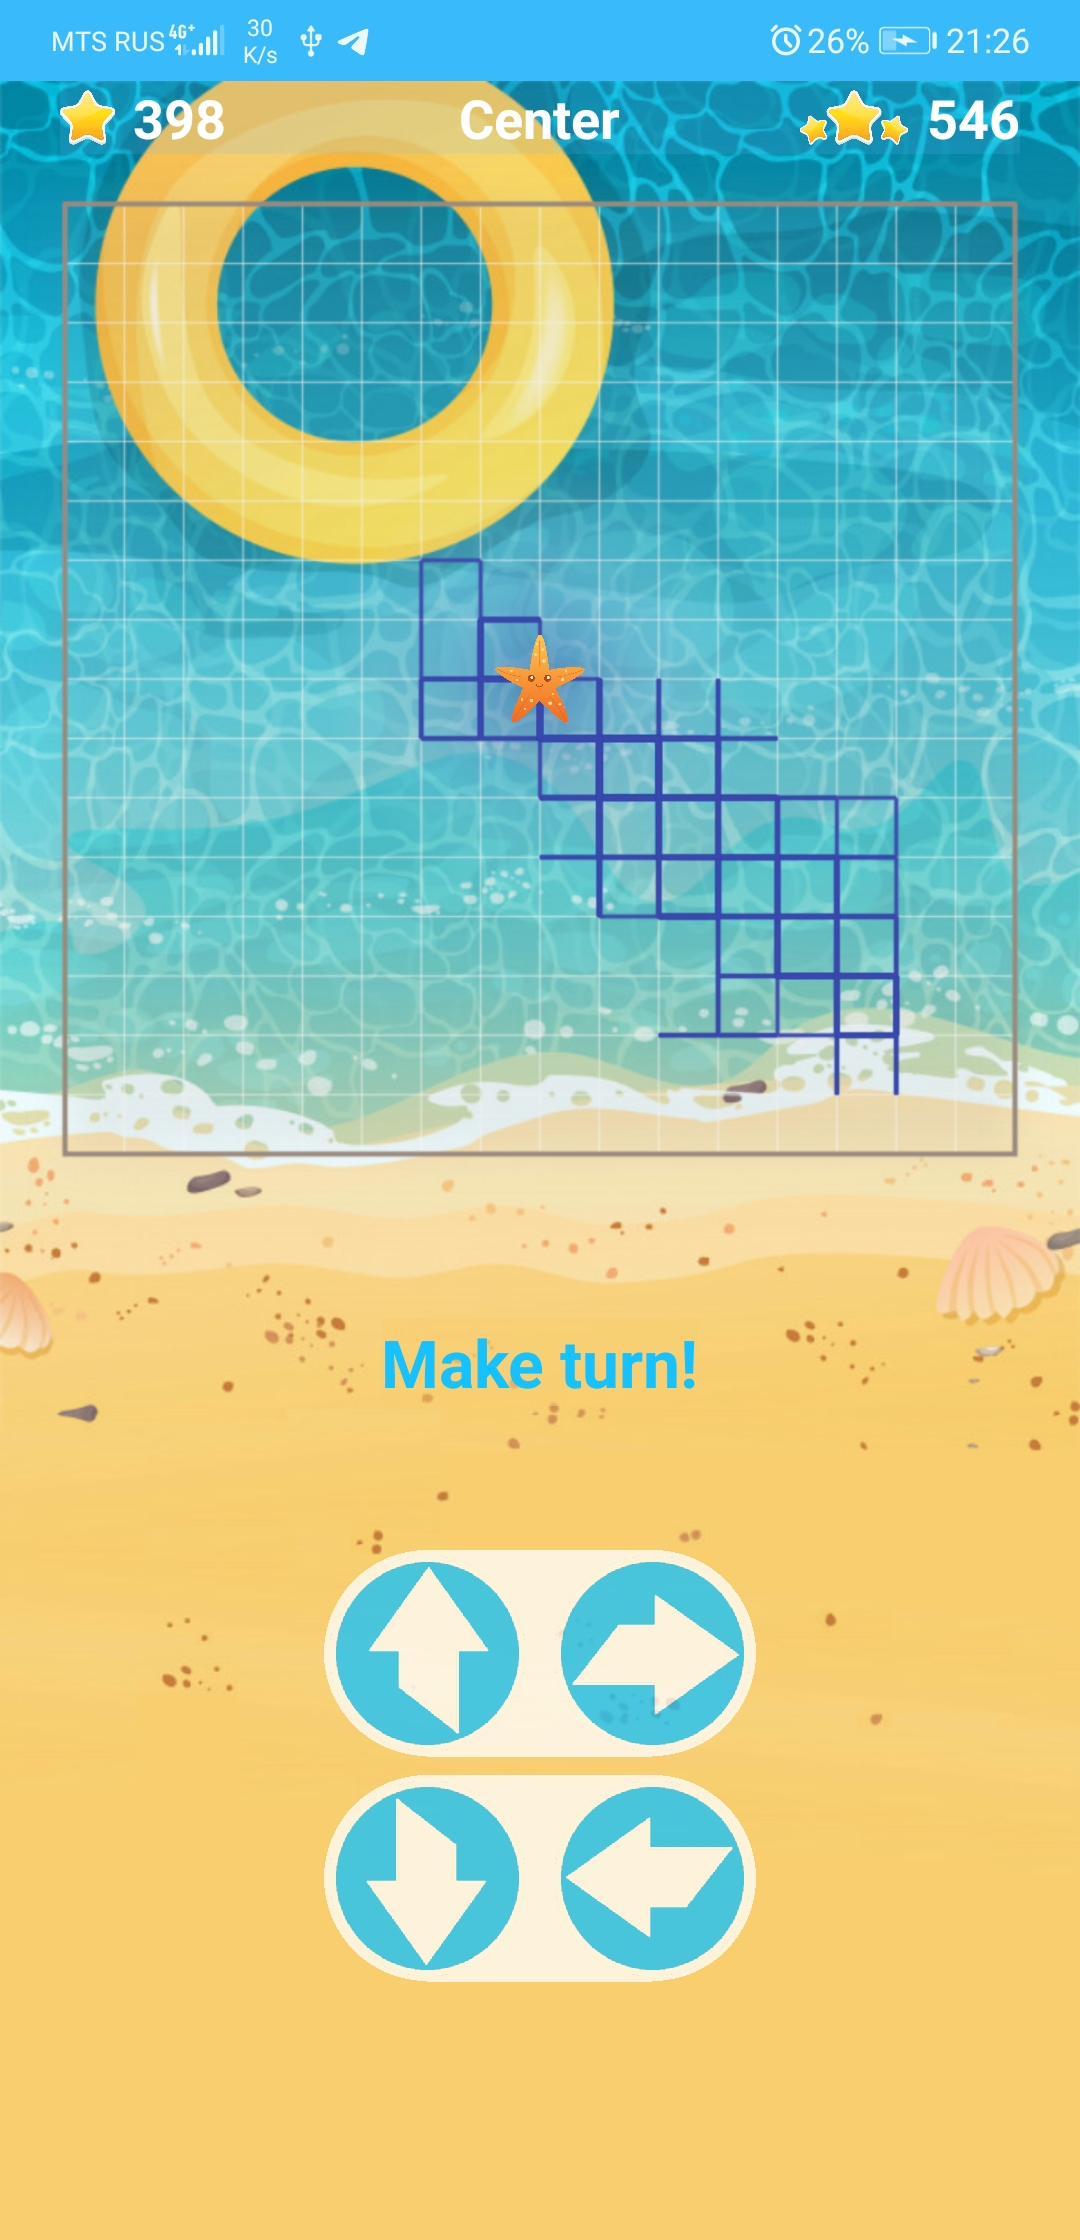
\includegraphics[scale=0.27]{screenshot_game_field}
    }
    \caption{
        Скриншот приложения Random Walk Game. Строка заголовка состоит из текущего количества ходов, 
        их целей и количества ходов в самой длинной игре. Игрок видит игровое поле, положение фишки и траекторию фишки. 
        Внизу экрана показана управляющая матрица $2$ на $2$, которая определяет результат совместного выбора стратегий игроками A и B. 
        Строки представляют собой возможный выбор стратегий для игрока A, а столбцы "--- для игрока B. Результирующее направление движения 
        определяется стрелкой в ячейке, расположенной в соответствующих строке и столбце.
    }\label{fig:screenshot_game_field}
\end{figure}


    
\begin{figure}[ht]
    \begin{minipage}[b][][b]{0.49\linewidth}\centering
        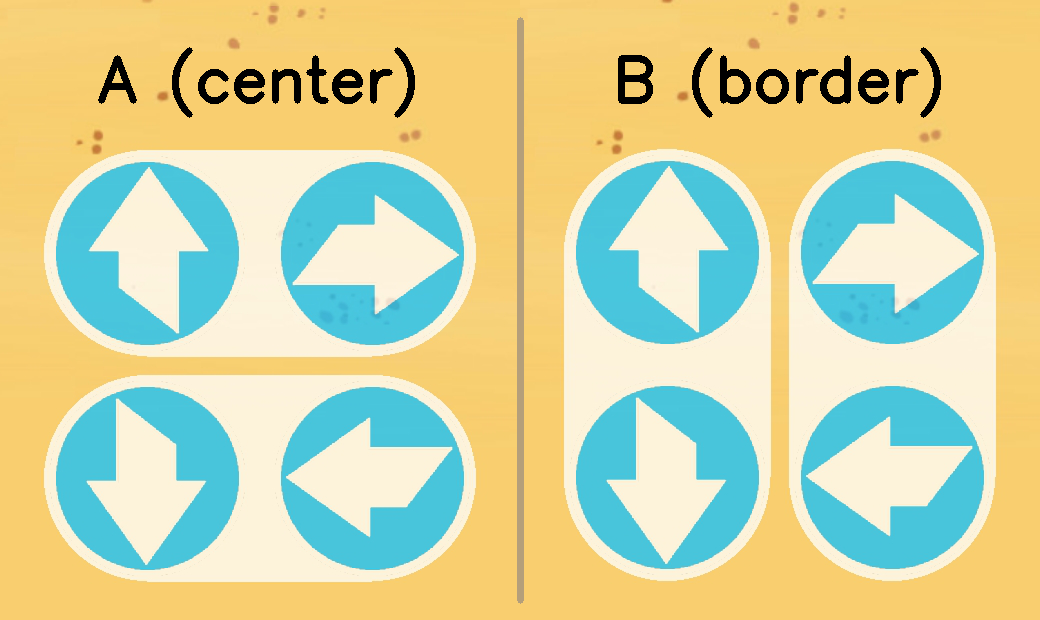
\includegraphics[width=0.5\linewidth]{controls} \\ а)
    \end{minipage}
    \hfill
    \begin{minipage}[b][][b]{0.49\linewidth}\centering
        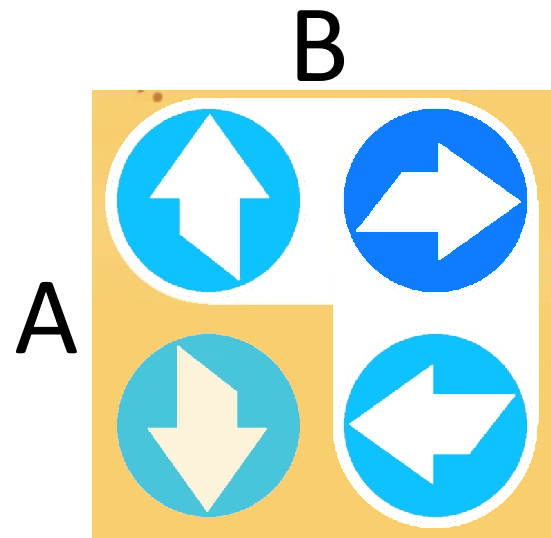
\includegraphics[width=0.5\linewidth]{fig1e} \\ б)
    \end{minipage}
    \caption{
        а) Кнопки управления для игрока А, целью которого является удержание фишки внутри поля как можно дольше (центр),
        и для игрока Б, целью которого является скорейшее достижение границы.
        б) Пример определения выбора результирующего движения фишки: игрок А выбрал первую строку (кнопку), ограничив движение направлениями вверх и вправо,
        игрок Б выбрал второй столбец, ограничив направления вправо и влево. В результате таких выборов игроков направление, которое выбрали оба игрока,
        оказывается на пересечении соответствующих столбца и строки, что дает итоговое направление движения "--- вправо.
    }\label{fig:controls}
\end{figure}


\section{Задачи, решаемые в диссертационном исследовании}\label{sec:ch1/sec3}

Разнообразие процессов случайных блужданий различной природы от бактерий и роботов до 
цен акций и игр, обуславливает наличие большого числа скрытых факторов, трудных для анализа в эксперименте.
Проведенный обзор показал наличие множества сложных экспериментов и соответствующих теоретических моделей,
аппроксимирующих поведение объектов на основе части выбранных признаков. В связи с этим для получения
всех преимуществ как теоретических основ анализа случайных блужданий, так и оценки соответствия экспериментального проведения
наиболее оптимальным стратегиям, необходимо сконструировать процесс, позволяющий собрать достаточное количество 
статистических данных для проведения анализа и учитывающий особенности влияния скрытых факторов на модель.

На основании выполненного обзора определим цель работы: получение информации о статистических
характеристиках процесса блужданий в ограниченной двухмерной области, индуцированного игровым
взаимодействием двух игроков-оппонентов и построение стохастической модели, способной воспроизвести эти характеристики.

Основные задачи диссертационного исследования:
\begin{itemize}
    \item Разработка стохастической модели блужданий на плоскости, управляемых
    игровым конфликтом, и получение характеристик игрового процесса.
    \item Разработка и имплементация алгоритмов для моделирования
    игровой пространственной динамики, используя стохастическую
    модель, получение информации о статистических характеристиках
    модельного процесса, таких как время достижения границы и его
    распределение.
    \item Реализация масштабной серии экспериментов с участием
    реальных игроков и получение статистически значимого массива
    данных.
    \item Исследование взаимосвязи результатов, полученных в ходе
    теоретического анализа, численного моделирования, и эксперимента, а
    также их совместная интерпретация.
\end{itemize}

\section{Выводы по главе 1}\label{sec:ch1/sec4}

В первой главе был проведён обзор предметной области и результатов
существующих исследований, посвящённых игровым взаимодействиям, случайным блужданиям,
Марковским цепям, а также теоретическому и экспериментальному способу анализа.
Используя проанализированные сведения была предложена новая специальная игровая динамика блужданий
на плоскости, управляемых игровым конфликтом двух игроков.

В главе рассмотрены антагонистические игры на примере задачи о разорении игрока, а также
продемонстрирована тесная взаимосвязь задачи с процессами случайных блужданий на отрезке.
Приведены работы обобщающие задачи о разорении игрока на многомерный случай нескольких игровых валют.
Рассмотрены приложения и задачи, при которых возникают процессы случайных блужданий, а также 
изучена информация о случайных полетах и выделен класс Марковских случайных процессов.
Проанализированы работы связывающие блуждания и игровую динамику, добавляющие случайную компоненту
в выбор игроков. Приведены теоретические исследования многошаговых игр на выживание.
Рассмотрен метод исследования с применением мобильных приложений для проведения полевых экспериментов.

В продолжение работы случайных блужданий игрового типа, сформулирована автором данной работы новая игровая механика, предлагаемая к исследованию. 
Приведено описание игры и визуализация мобильного приложения, используемого для проведения полевого эксперимента.

На основе проведенного обзора научных работ определена цель диссертационного исследования как
получение информации о статистических характеристиках процесса блужданий в ограниченной двухмерной области, индуцированного игровым
взаимодействием двух игроков-оппонентов и построение стохастической модели, способной воспроизвести эти характеристики.








